\chapter{Evaluaciones y análisis de resultados}
\label{results}

\section{Estimación del parámetro Beta}
% PRIMERO EXPLICAR COMO DEPENDE LA EJECUCION CON EL PARÁMETRO BETA
% PARA VALORES MAS CHICOS ...
% PARA VALORES MAS GRANDES...
% DAR UNA IDEA DEL RANGO DE VALORES BETA DE ACUERDO A LA ECUACION, PARA DIFERENCIAS DE SCORE = 1
% MOSTRAR GRAFICO/S DE RELACION ENTRE 
% POR LO TANTO, UN PARAMETRO QUE TIENE EN CUENTA ESTOS ASPECTOS, QUE PODRIA EVALUAR CORRECTAMENTE LA EJECUCION EN FUNCION DE BETA , Y QUE ADEMAS ES EL DATO MAS IMPORTANTE EN LA EJECUCION ES EL TIEMPO DE EJECUCION

En las secciones previas hemos propuesto un método de diseño que se basa en búsqueda estocástica sobre el espacio de secuencias.
El método de búsqueda es guiado por el resultado de una función que asigna un puntaje a cada secuencia, el cual resulta siempre mayor o igual a 0.

La secuencia resultante buscada se caracteriza por tener un puntaje igual a 0, por lo tanto, el método puede verse como la búsqueda de un mínimo global sobre la superficie
que relaciona cada posible secuencia con su valor de puntaje.
A pesar que, previo a desarrollar la aplicacion asumimos que el espacio de soluciones era considerablemente grande, no sabemos como es exactamente esta superficie cada secuencia con el puntaje que definimos.
El valor(o el rango) óptimo para el parámetro que Beta depende en gran parte de las características de esta superficie.
% De estas característica depende en gran parte el valor óptimo de beta. 

Un valor de beta mayor permite la exploracion de superficies que requieren superar mínimos locales para alcanzar secuencias con puntaje 0.
Un valor de beta mas chico representa recorrer un camino más directo hacia el mínimo pero, si la superficie es rugosa, podría requerir la evaluacion de una gran cantidad de posibilidades.
Incluso, si la búsqueda se estanca en un mínimo local, un valor muy chico de beta solo podría encontrar la solución en un tiempo infinitamente grande(la probabilidad de aceptación nunca es 0, por lo tanto no es imposible encontrar el resultado si es que existe).

En esta aplicación, además, partiendo de una secuencia inicial dada por el usuario, resultaría mejor obtener la secuencia con puntaje mínimo que esté más cerca en la superficie, es decir, que sea más similar a la secuencia inicial.
Esto implica una menor cantidad de mutaciones, lo que equivale a un valor de beta mas chico.




% Una superficie de búsqueda con más cantidad de mínimos locales(y más profundos) requerirá un valor de Beta mayor para poder sobrepasar fácilmente estos durante la búsqueda, 
% mientras que una superficie mas lisa con un mínimo global más marcado, probablemente aprovechará la explotación local que puede proveer un valor de Beta más chico. 
% Dadas las características estocásticas de la búsqueda, la definición de valores/rangos óptimos se refiere al promedio del tiempo de búsqueda y no a la comparación entre dos ejecuciones puntuales.
% 
% En nuestro caso, las propiedades de la superficie de búsqueda están dadas por la función que relaciona el espacio de secuencias y el puntaje resultante del conjunto de evaluaciones detallado previamente.
% Esta función, y por lo tanto la superficie resultante, no sólo no se conocen sino que, además, variarán al modificar el subconjunto de herramientas que se utilizan durante las evaluaciones y/o al cambiar los parámetros de éstas.
% En primer lugar, entonces, se debe hacer una estimación del rango óptimo de valores de beta, tal que la búsqueda sea 
% 
% En nuestro caso, la búsqueda se realiza mediante mutaciones puntuales sobre la secuencia.
% El valor de beta, como se describió en las secciones previas, relaciona el porcentaje de aceptacion de una mutación con una diferencia en el score evaluado.
% % Para una misma diferencia
% Por ejemplo, para una diferencia de 1 en el puntaje, el porcentaje de aceptacion ....varia entre .....
% 

Inicialmente no tenemos ningún conocimiento de como se relaciona el valor de beta con la ejecución resultante, para tener una primera idea global de esta dependencia analizamos las ejecuciones de 6 corridas independientes.
3 de estas corridas se realizaron a partir de secuencias random, mientras que otras 3 se inician a partir de secuencias naturales definidas(distintas entre si).
En todos los casos la longitud de la secuencia fue de 30 aminoácidos.
Este mismo esquema de 6 corridas se repitio para valores de beta = 0.5 y 2.4. 
En el caso de beta más chico(0.5), la probabilidad de aceptar una mutación para una diferencia de 1 en el puntaje es de ........, 
Para el beta más grande(2.4), la probabilidad de aceptar una mutación para una diferencia de 1 en el puntaje es de ........
% Los resultados de las corridas se muestran en la tabla ......... ***CONVIENE RESUMIR BIEN LOS DATOS EN UNA TABLA? EL UNICO DATO CREO QUE SERIA EL TOTAL DE ITERACIONES

En el grafico \ref{fig:scoreVsiter}
% GRAFICO DE SCORE vs ITERACION   (MEDIAS Y StdDeV COMPLETO HASTA EL FINAL)   +  CORRIDAS INDIVIDUALES
se muestra la dependencia del puntaje con las iteraciones, tanto el promedio(y desviacion estandar) para todas las ejecuciones mencionadas(grafico refA), como el detalle de las ejecuciones individuales.
El perfil que se muestra permite aclarar mejor los conceptos mencionados previamente. 
Se ve claramente que hay una diferencia en el orden de magnitud de la cantidad de iteraciones que alcanzan las corridas ejecutadas utilizando el valor de beta mayor.
Un valor mayor de beta realiza una mayor exploración del espacio de soluciones, lo que se ve reflejado en un rango mucho mayor de mutaciones aplicadas(las ejecuciones llegan a >2000 iteraciones).
Un valor de beta menor solo acepta un número chico de mutaciones que no reduzcan el puntaje, y por lo tanto 
% PONER ALGUNA CONCLUSION DE QUE DICE ESTO ACERCA DE LA SUPERFICIE 

% En primer lugar vemos que, al menos para estas ejecuciones, siempre se encontraron resultados deentro de los limites de iteraciones impuestos por la implementación(ver.... ), tanto para el valor de beta mas chico como para el valor de beta mayor.
% En las primeras iteraciones el valor de score es alto, es fácil que cualquier mutación dirigida pueda bajar este valor de score y esto se ve reflejado en una caída rapida del score y un reducido número de intentos de mutación.


% Vemos que el resultado es alcanzable tanto para valores chicos de beta como para valores grandes, y que para el valor más chico se 
Vemos que para el valor de beta chico siempre se encuentra un resultado en una cantidad relativamente baja de mutaciones,
esto parece indicar que hay un camino que conduce desde cada punto de inicio hacia un resultado bajando siempre el valor de score, es decir, sin atravesar ninguna barrera.



\begin{figure} 
\advance\leftskip-2cm
\subfigure[Ejecuciones individuales]{\label{fig:scoreVsiter-a}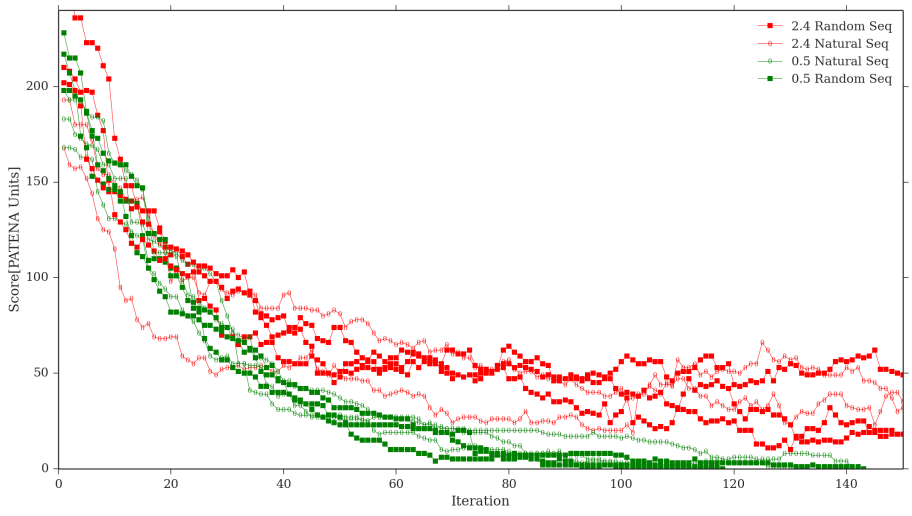
\includegraphics[width=1.15\textwidth]{img/resultados/individuales-scoreVsiter-hasta150.png}}
\subfigure[Valores medios y desviaciones]{\label{fig:scoreVsiter-b}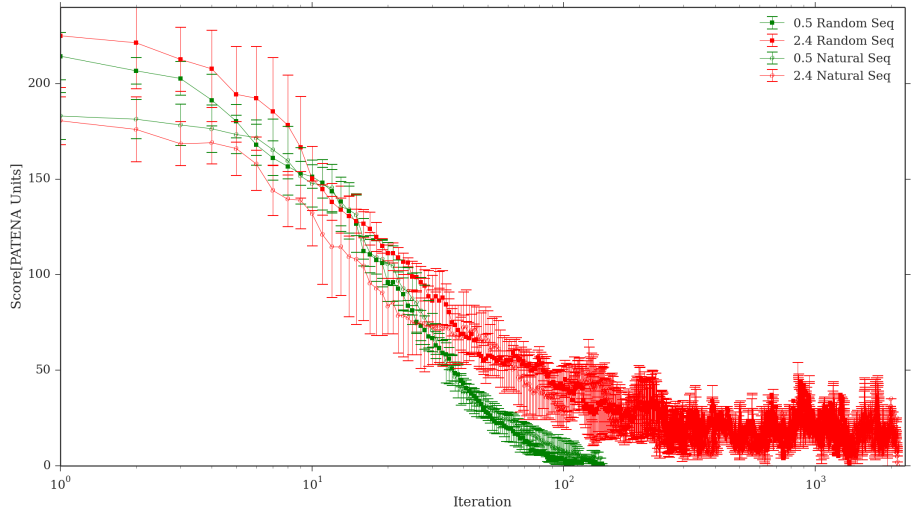
\includegraphics[width=1.15\textwidth]{img/resultados/scoreVsiter-cada1-hasta2270.png}}
% \begin{subfigure}
% \begin{center}
% \centering
% \includegraphics[width=1.15\textwidth]{it}
% 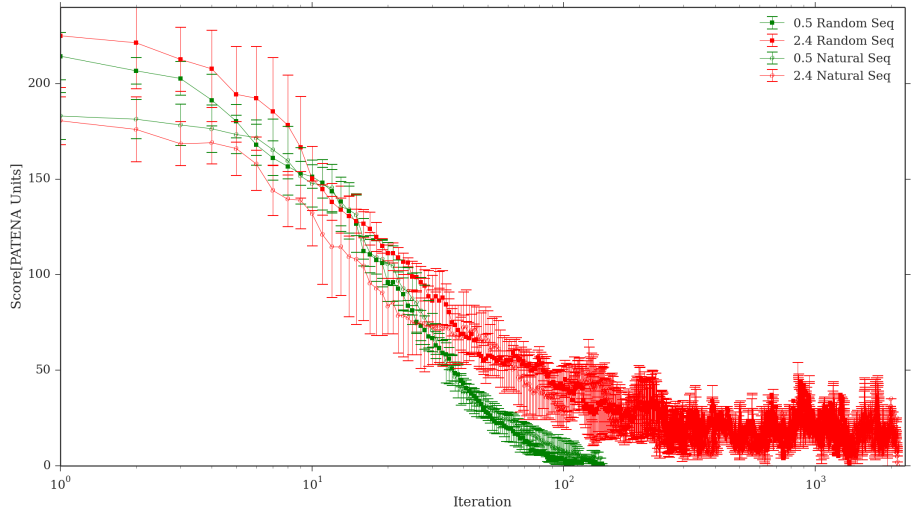
\includegraphics[width=1.15\textwidth]{img/resultados/scoreVsiter-cada1-hasta2270.png}
% \end{center}
%  \caption{}
%  \label{fig:scoreVsiter-mean}
% \end{subfigure}
% \begin{subfigure}[h!]]{0.3\textwidth}
% \advance\leftskip-2cm
% \begin{center}
% \centering
% 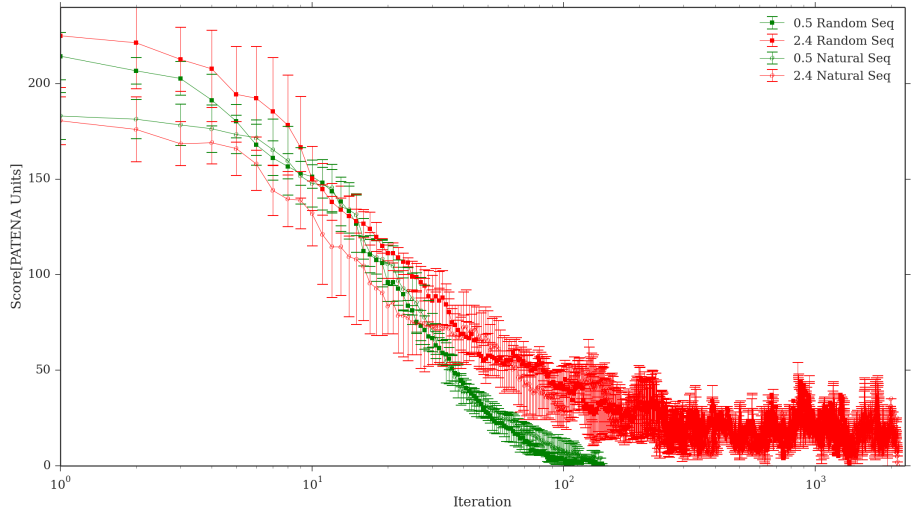
\includegraphics[width=1.15\textwidth]{img/resultados/scoreVsiter-cada1-hasta2270.png}
% \end{center}
 \caption{Puntaje asociado a cada iteración}
 \label{fig:scoreVsiter}
% \end{subfigure}
\end{figure}



Esta es, sin embargo, una vista muy general de la ejecución. 
Para tener una idea mas detallada es necesario ver otros parámetros relevantes de la ejecución
En el grafico....% y   MUT-ATTEMPTS vs ITERACION (MEDIAS Y StdDeV COMPLETO HASTA EL FINAL)   +  CORRIDAS INDIVIDUALES
se muestra el número de intentos de mutacion promedio asociado a cada valor de beta.
De nuevo, mostramos los valor promedios(y sus desviaciones correspondientes) para todas las ejecuciones, y la primera parte de las ejecuciones individuales.
Vemos que el reducido número de iteraciones que resulta de un valor bajo de beta se produce a costas de una cantidad más elevada de intentos de mutaciones, sobre todo en las .
% Esto, sin embargo, no implica que esta sea la búsqueda optima, ya que encontrar este camino puede requerir evaluar una gran cantidad de otros caminos posibles, es decir, intentar otras mutaciones.
% Para tener una idea de que tan dificil es encontrar este camino, vemos en el gráfico %ref. grafico intentos mutacion VS iteracion
% la cantidad de intentos de mutación para corridas iniciando desde     ...........  utilizando los mismos valores de beta que antes.
% Como se ve, para valores mas chicos de beta se requiere un mayor numero de intentos de mutacion hasta encontrar una propuesta que que sea aceptada, 
% mientras que para el valor de beta mayor es más fácil que se acepte una propuesta de mutación,
% ya sea porque disminuye el puntaje o porque la probabilidad de aceptación lo permite. 
Sin embargo, no sabemos como estos intentos afectan a la búsqueda global.
% Todavía no sabemos las implicancias de realizar esta cantidad de intentos de mutacion sobre la búsqueda.
Para conocer cual es el rango(o valor) óptimo de beta utilizamos como variable de evaluación al tiempo de ejecución. 
Este valor es directamente proporcional a la cantidad total de mutaciones aceptadas que se necesitan y la cantidad de mutaciones que se intentan.
Por lo tanto, la estimación del valor de beta que provea un menor tiempo de ejecución nos permite conocer cual es el valor de beta que provee un correcto balance entre la exploración y la explotación de la superficie.


\begin{figure} 
\advance\leftskip-2cm
\subfigure[Ejecuciones individuales]{\label{fig:mutAttemptsVsite-a}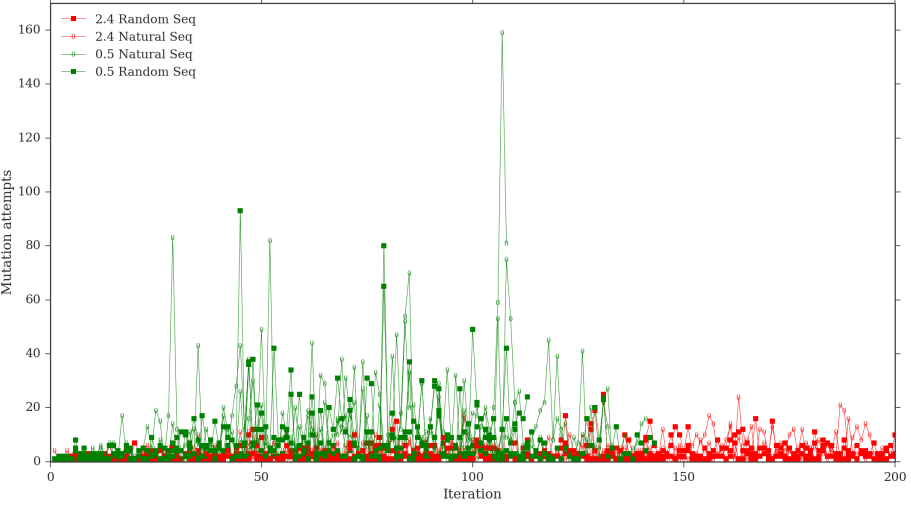
\includegraphics[width=1.15\textwidth]{img/resultados/individuales-mutAt-vs-iter-hasta200.png}}
\subfigure[Valores medios y desviaciones]{\label{fig:mutAttemptsVsite-b}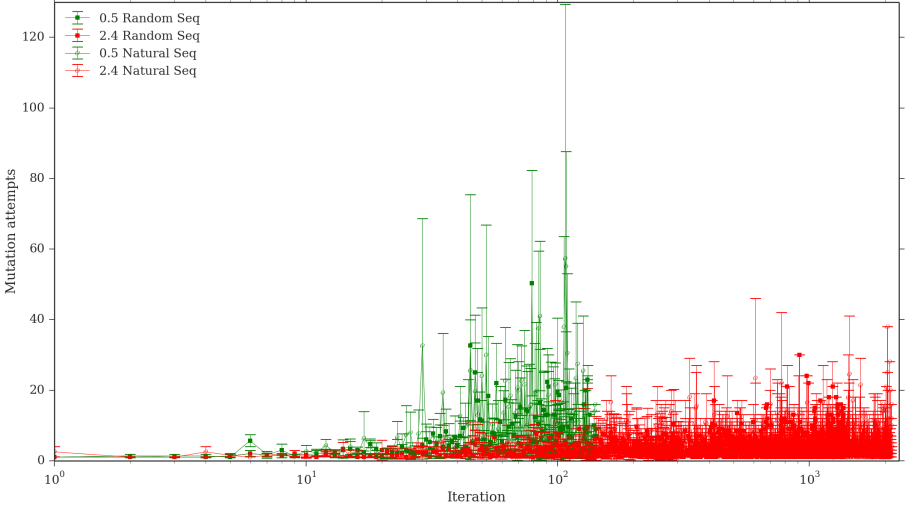
\includegraphics[width=1.15\textwidth]{img/resultados/mutAttemptsVsite-cada1-hasta2270.png}}
\caption{Dependencia del número de intentos de mutación con la iteración}
\label{fig:mutAttemptsVsite}
\end{figure}

%  Si la superficie requiere de una mayor exploración, entonces un valor de beta muy chico podría no resultar en una búsqueda optima , incluso no llegando nunca a un resultado(quedando estancado en un mínimo local).
% De esta forma, valores mayores permiten facilmente aceptar una mutacion que permite luego pasar entre dos puntos que pueden estar incluidos en minimos locales separados. 
% Esto permite explorar superficies más amplias. 


% El valor de beta, entonces, permite balancear entre el número de iteraciones(es decir, las mutaciones aceptadas) y el número de intentos de mutación.  
% Para evaluar correctamente cómo la ejecución global depende del valor de beta se utiliza el tiempo total de ejecución. 
% El correcto balance entre mutaciones evaluadas y aceptadas dara un menor número total de secuencias evaluadas hasta llegar al mínimo y, por lo tanto, un menor tiempo de ejecución. 
% Como variable para evaluar la relación entre los diferentes valores de Beta se analiza el tiempo de ejecución. 
% Este valor es proporcional al total de evaluaciones que se realizaron sobre la secuencia



\section{Tiempo de ejecución correspondiente}

% RESULTANDOS DE TIEMPO EN FUNCION DE LONGITUD
Ahora que tenemos fijado un valor para el parámetro $\beta$ y tenemos un conjunto definido de herramientas de evaluación
Una vez definido el valor de beta que dará el correcto balance entre intentos de mutación y mutaciones aceptadas, queremos saber como se traduce esto en un tiempo de ejecución concreto.
Se realizan entonces evaluaciones del tiempo de ejecución en función de la longitud de la secuencia, lo que nos dará una idea del orden de tiempo que demora las ejecuciones y como éste varía con la longitud.
% Utilizando los parámetros estándar, el tiempo de ejecución solo varía con la longitud de la secuencia. 






\section{Análisis de diseños resultantes}

% DIVERGENCIA EN EL CONJUNTO DE RESULTADOS

Ahora que tenemos fijados todos los aspectos de ejecución del método de diseño y que, efectivamente, podemos obtener diseños con los requerimientos estándar en un tiempo relativamente corto, 
queremos conocer más acerca de los diseños resultantes que provee.  
Hasta el momento vimos el proceso de ejecucion analizando de forma abstracta la iteraciones como mutaciones aceptadas, sin embargo, no sabemos como se distribuyen estas mutaciones sobre la secuencia y cómo, el resultado de esto, 
afecta las características secuenciales de los resultados.
Para analizar las propiedades de los resultados se realizaron ejecuciones a partir de una misma secuencia inicial.  
En total se realizaron 74 corridas individuales.

Inicialmente no tenemos ningún conocimiento sobre cómo estan 

\begin{figure}[htbp]
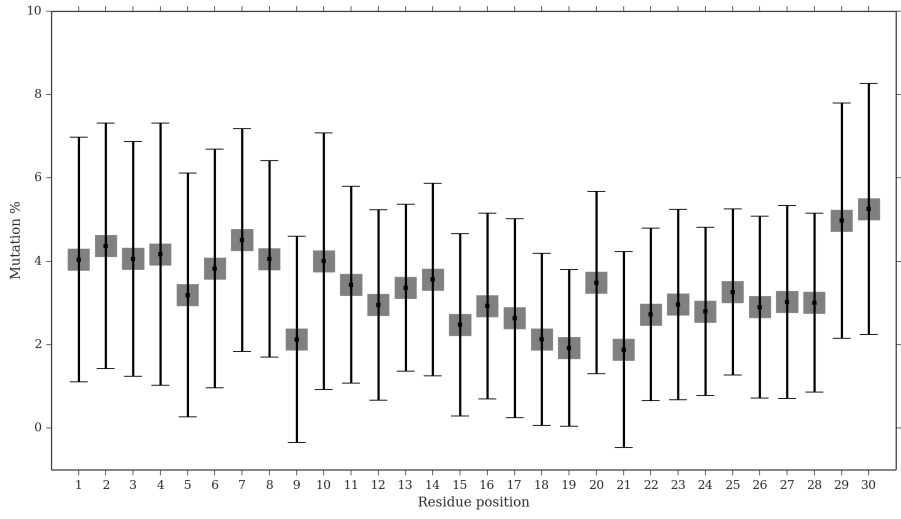
\includegraphics[width=\textwidth]{img/resultados/mutationsPerPosition.png}
\caption{Procentaje medio de mutaciones para cada posición en 74 corridas individuales}
\label{fig:mutationPerSite}
\end{figure}

Por definición del método de diseño, sabemos que los resultados tendrán las propiedades buscadas y no tendrán las propiedades negativas, pero, hasta el momento, no sabemos nada más acerca de sus propiedades secuenciales.
Teniendo en cuenta los fundamentos del método, que describen a las secuencias buscadas como un conjunto amplio y complejo, esperamos obtener un 




\begin{figure}[htbp]
% \advance\leftskip-2cm
\centering
\subfigure[b][Identidad entre las secuencias resultantes(74) y la secuencia inicial]{\label{fig:identity-a}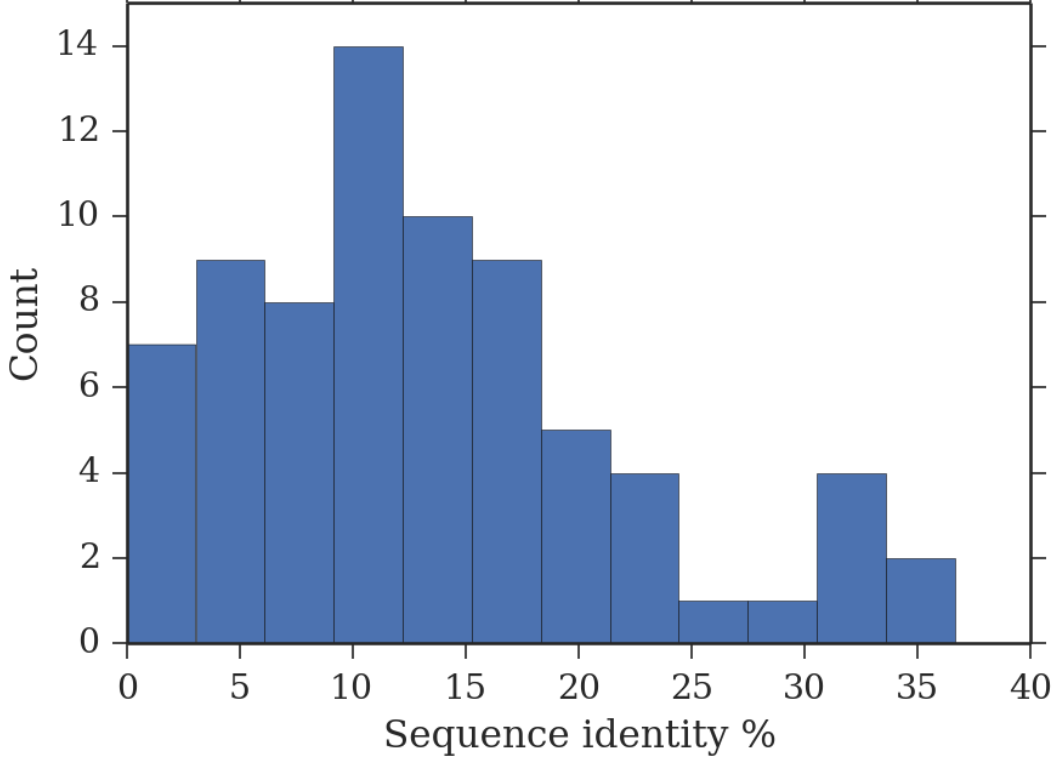
\includegraphics[width=0.7\textwidth]{img/resultados/againstStartSeq-74.png}}
\subfigure[b][Identidad entre cada par posible de secuencias resultantes(74*74)]{\label{fig:identity-b}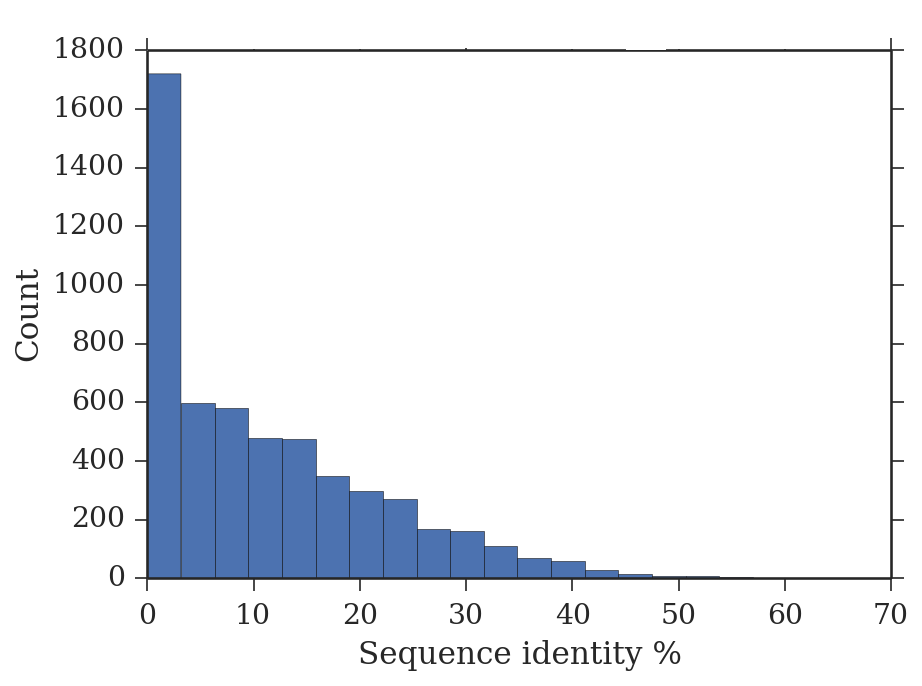
\includegraphics[width=0.7\textwidth]{img/resultados/againstAll-74-borrado.png}}
\caption{Histograma de identidad de las secuencias resultantes}
\label{fig:identity}
\end{figure}
% 
% \begin{figure}[htbp]
% 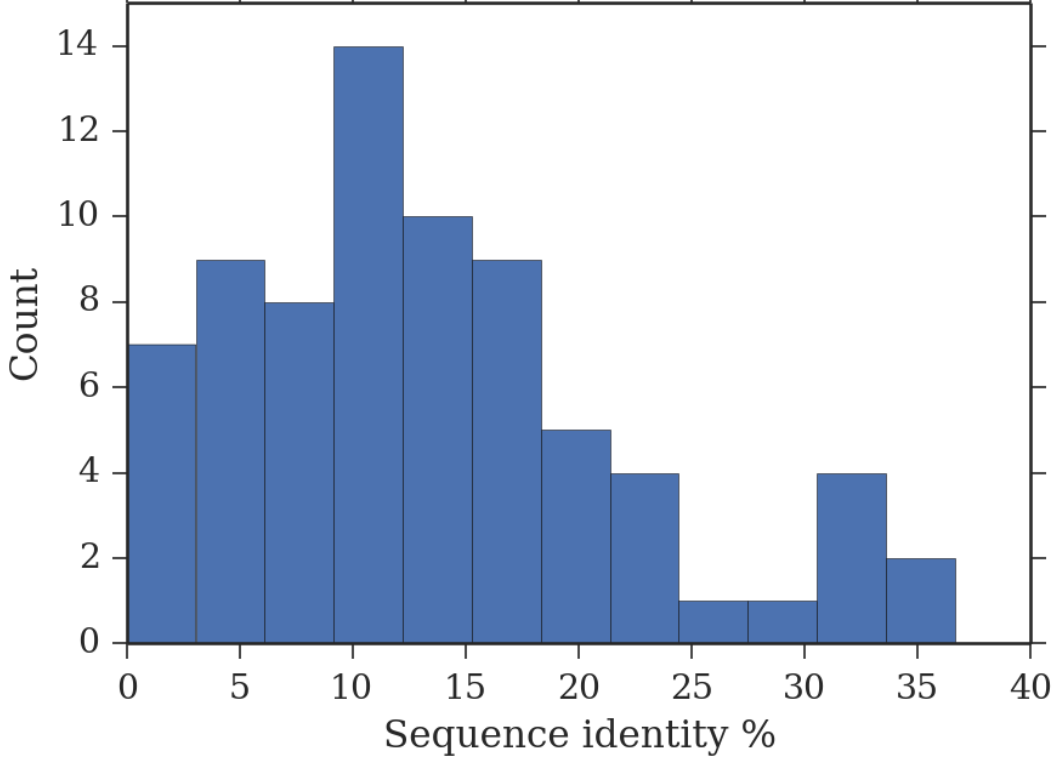
\includegraphics[width=\textwidth]{img/resultados/againstStartSeq-74.png}
% \caption{Histograma de identidad entre las secuencias resultantes(74) y la secuencia inicial}
% \label{fig:identityVsInitialSeq}
% \end{figure}


% \begin{figure}[htbp]
% 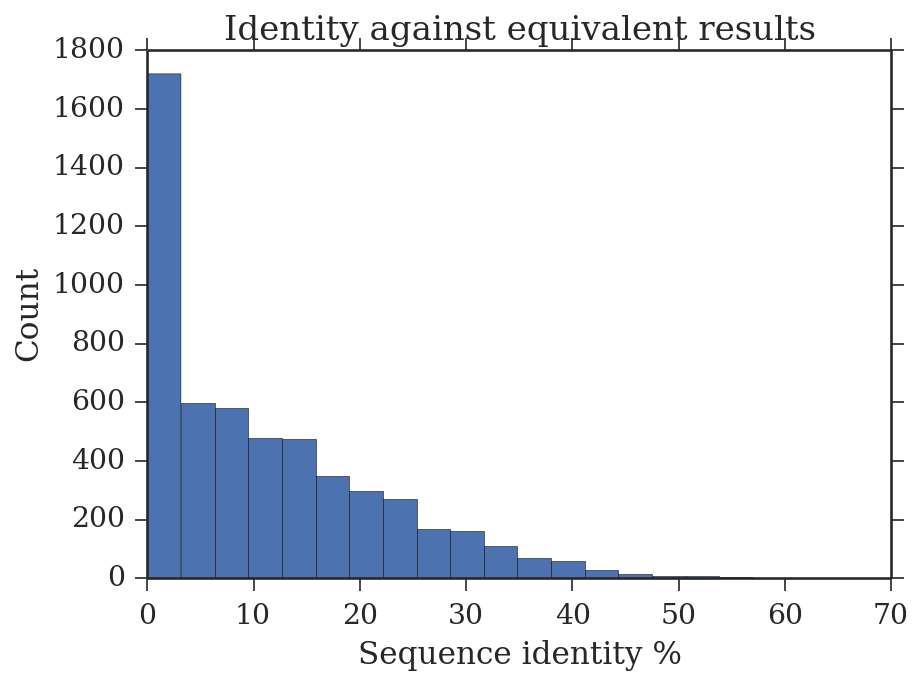
\includegraphics[width=\textwidth]{img/resultados/againstAll-74.png}
% \caption{Histograma de identidad entre cada par posible de secuencias resultantes(74*74)}
% \label{fig:identityVsAll}
% \end{figure}


\begin{figure}[htbp]
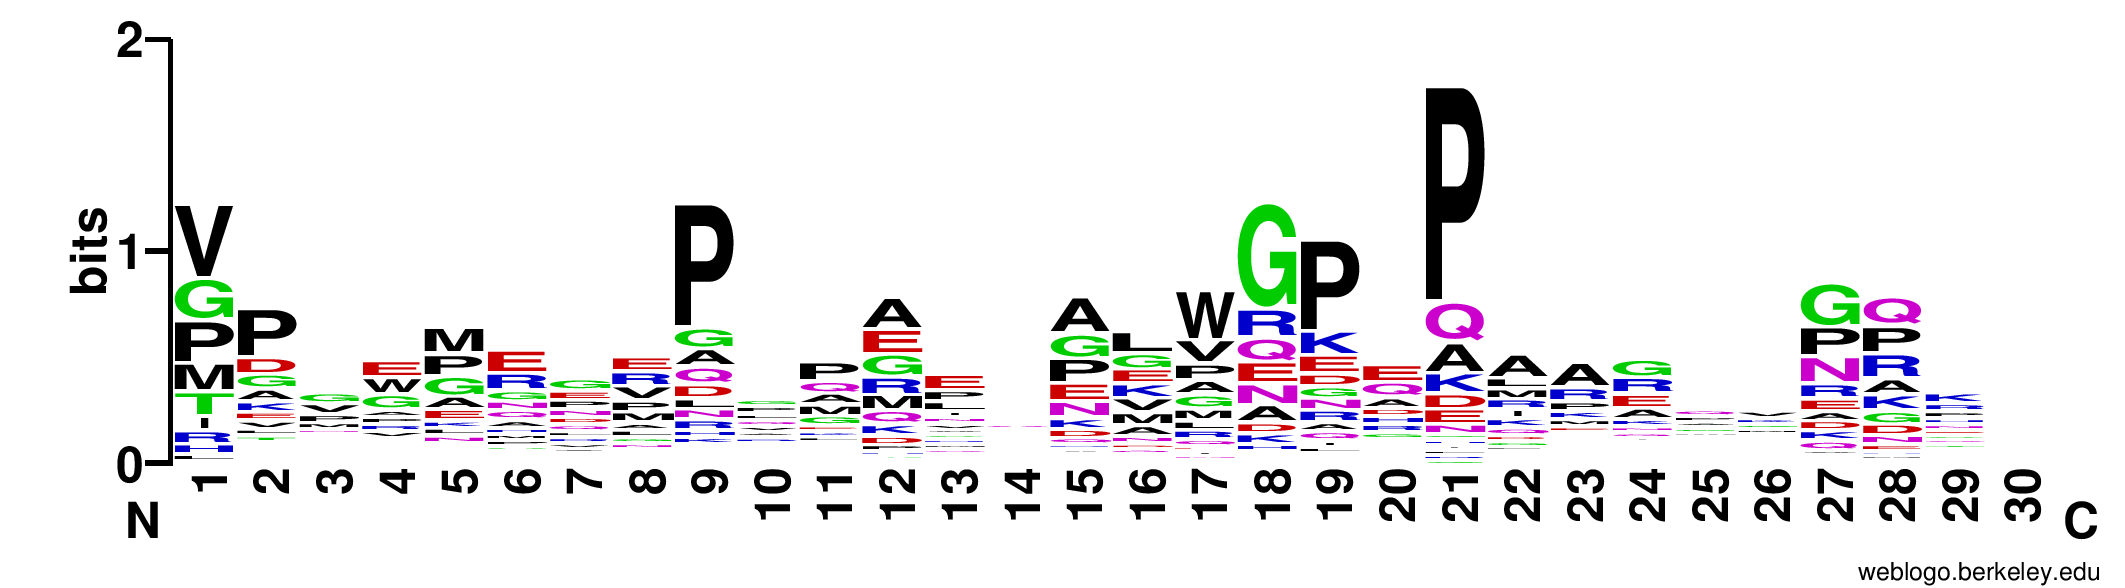
\includegraphics[width=\textwidth]{img/resultados/logo.png}
\caption{}
\label{fig:logo}
\end{figure}